% ============================================================
%  第七章（续）  7.3—7.5 节
%  接 ch07a.tex，故不含 \chapter
% ============================================================
\providecommand{\cfs}{\mathrel{\square\!\!\rightarrow}}

\section{公理化刻画}

公理在形式系统的刻画中起着重要作用。它们以经济的方式描述系统的本质性质，从而使不同的表述方式可以相互比较，也使等价性或包含关系易于检验。此外，公理常常可以用作推理规则，从一组给定前提推出（或验证）新的关系。在下一小节中，我们将建立一组公理，刻画递归系统与非递归系统中形如 $Y_x(u)=y$ 的反事实语句之间的关系。随后（\S 7.3.2）我们用这些公理演示：因果效应的可识别性可以借助符号手段来验证，其做法与第三章（\S 3.4）的推导平行。最后，\S 7.3.3 为因果相关性这一概念建立公理，并与刻画信息相关性的公理相对照。

\subsection{结构反事实的公理}

我们给出反事实的三条性质——复合性（composition）、实效性（effectiveness）与可逆性（reversibility）——它们在一切因果模型中成立。

\medskip
\noindent\textbf{性质 1（复合性）}\quad 对因果模型中任意三组内生变量 $X$、$Y$ 与 $W$，有
\begin{equation}
W_x(u)=w\ \Longrightarrow\ Y_{xw}(u)=Y_x(u). \tag{7.19}
\end{equation}

复合性是说：若我们把变量 $W$ 强制设为它在没有我们干预时本会取的值 $w$，那么这一干预对系统中其他变量没有影响。该不变性在一切固定条件 $\doop(X=x)$ 下都成立。

由于复合性允许消去一个下标（即把 $Y_{xw}(u)$ 约简为 $Y_x(u)$），我们需要为下标集为空的变量给出解释；自然地，我们把它等同于未受任何干预时的变量。

\begin{definition}[空行动]
\[
Y_\varnothing(u)\triangleq Y(u).
\]
\end{definition}

\begin{corollary}[一致性]
对因果模型中任意变量集 $Y$ 与 $X$，有
\begin{equation}
X(u)=x\ \Longrightarrow\ Y(u)=Y_x(u). \tag{7.20}
\end{equation}
\end{corollary}

\begin{proof}
在式 \textup{(7.19)} 中以 $X$ 代 $W$、以 $\varnothing$ 代 $X$，得
\[
X_\varnothing(u)=x\ \Longrightarrow\ Y_{\varnothing x}(u)=Y_\varnothing(u).
\]
空行动（定义 7.3.1）允许我们删去 $\varnothing$，于是左端化为 $X(u)=x$、右端化为 $Y_x(u)=Y(u)$。
\end{proof}

\textup{(7.20)} 中的蕴含关系被 Robins (1987) 称为“一致性”。\footnote{一致性与复合性在经济学（Manski 1990; Heckman 1996）与统计学（Rosenbaum 1995）的潜在结局框架（\S 3.6.3）中被例行使用。一致性由 Gibbard and Harper (1976, p.~156) 与 Robins (1987) 正式表述（见式 \textup{(3.52)}）；复合性见于 Holland (1986, p.~968)，并由 J. Robins 提请我注意。}

\medskip
\noindent\textbf{性质 2（实效性）}\quad 对任意变量集 $X$ 与 $W$，$X_{xw}(u)=x$。

实效性刻画干预对被操纵变量本身的效果——即：若我们强制变量 $X$ 取 $x$，则 $X$ 确实会取 $x$。

\medskip
\noindent\textbf{性质 3（可逆性）}\quad 对任意两个变量 $Y$ 与 $W$、以及任一变量集 $X$，
\begin{equation}
\bigl(Y_{xw}(u)=y\bigr)\ \&\ \bigl(W_{xy}(u)=w\bigr)\ \Longrightarrow\ Y_x(u)=y. \tag{7.21}
\end{equation}

可逆性排除了反馈环导致的多重解。若把 $W$ 设为 $w$ 会使 $Y$ 取值 $y$，而把 $Y$ 设为 $y$ 又会使 $W$ 取到 $w$，则 $W$ 与 $Y$ 会自然地（分别）取 $w$ 与 $y$，无须任何外部设定。

在递归系统中，可逆性直接由复合性推出。这很容易看出：在递归系统中，$Y_{xw}(u)=Y_x(u)$ 与 $W_{xy}(u)=W_x(u)$ 二者必居其一。于是可逆性约化为
\[
\bigl(Y_{xw}(u)=y\bigr)\ \&\ \bigl(W_x(u)=w\bigr)\ \Longrightarrow\ Y_x(u)=y
\]
（复合性的另一形式），或约化为
\[
\bigl(Y_x(u)=y\bigr)\ \&\ \bigl(W_{xy}(u)=w\bigr)\ \Longrightarrow\ Y_x(u)=y
\]
（平凡为真）。

可逆性反映了“无记忆”行为：系统的状态 $V$ 追踪 $U$ 的状态，而与 $U$ 的历史无关。一个典型的不可逆例子，是两位奉行“针锋相对”策略的当事人所构成的系统（如囚徒困境）。在相同的外部条件 $U$ 下，该系统有两个稳定解——合作与背叛——因而不满足可逆性条件：强制任一方合作会导致另一方合作（$Y_w(u)=y$，$W_y(u)=w$），但这并不保证一开始就合作（$Y(u)=y$，$W(u)=w$）。在这类系统中，不可逆是状态描述过于粗糙的产物：并非所有决定系统最终状态的因素都被纳入 $U$。在针锋相对的系统中，完备的状态描述应包含当事人此前的行动等因素；一旦补入这些缺失因素，可逆性便恢复。

一般而言，复合性、实效性与可逆性三者相互独立——没有一条是另外两条的推论。这可以通过构造使其中两条成立而第三条不成立的具体模型来证明（Galles and Pearl 1997）。在递归系统中，复合性与实效性相互独立，而可逆性如前所示平凡成立。

下一定理断言性质 1—3 的可靠性，即它们的有效性。

\begin{theorem}[可靠性]
复合性、实效性与可逆性在结构模型语义中是可靠的；也就是说，它们在一切因果模型中成立。
\end{theorem}

定理 7.3.3 的证明见 Galles and Pearl (1997)。

下一定理确立这三条性质作为公理或推理规则时的完备性。完备性即充分性：反事实语句的一切其他性质都可从这三条推出。完备性的另一种解释是：给定任一与性质 1—3 相容的反事实语句集 $S$，都存在一个因果模型 $M$，使 $S$ 在其中为真。

完备性的形式证明要求阐明两个技术性质——存在性与唯一性——它们隐含在因果模型的定义（定义 7.1.1）之中。

\medskip
\noindent\textbf{性质 4（存在性）}\quad 对任意变量 $X$ 与变量集 $Y$，
\begin{equation}
\exists x\in X\ \ \text{s.t.}\ \ X_y(u)=x. \tag{7.22}
\end{equation}

\medskip
\noindent\textbf{性质 5（唯一性）}\quad 对每个变量 $X$ 与变量集 $Y$，
\begin{equation}
X_y(u)=x\ \&\ X_y(u)=x'\ \Longrightarrow\ x=x'. \tag{7.23}
\end{equation}

\begin{definition}[递归性]
设 $X$ 与 $Y$ 为模型中的单变量，并令 $X\to Y$ 表示：对 $x$、$w$ 与 $u$ 的某些取值，有 $Y_{xw}(u)\ne Y_w(u)$。若对任意序列 $X_1,X_2,\dots,X_k$，都有
\begin{equation}
X_1\to X_2,\ X_2\to X_3,\ \dots,\ X_{k-1}\to X_k\ \Longrightarrow\ X_k\nrightarrow X_1, \tag{7.24}
\end{equation}
则称模型 $M$ 是递归的。
\end{definition}

显然，凡因果图 $G(M)$ 无环的模型 $M$ 必为递归的。

\begin{theorem}[递归完备性]
复合性、实效性与递归性构成完备的公理系统（Galles and Pearl 1998; Halpern 1998）。\footnote{Galles and Pearl (1997) 在如下假设下证明了递归完备性：对任意两个变量，人们知道其中哪一个（若存在）是另一个的祖先。Halpern (1998) 在没有这一假设的条件下证明了递归完备性，只要求对模型中的任意两个变量已知式 \textup{(7.24)} 成立。Halpern 还针对 $Y_x(u)$ 的解不唯一或不存在的情形给出了一组公理。}
\end{theorem}

\begin{theorem}[完备性]
复合性、实效性与可逆性对一切因果模型构成完备的公理系统（Halpern 1998）。
\end{theorem}

可靠性与完备性的实际意义，在我们试图检验某组条件是否足以识别某个反事实量 $Q$ 时便显现出来。就此而言，可靠性保证：若我们用这三条公理对 $Q$ 作符号演算，并成功把它约化为一个只含普通概率（不含反事实项）的表达式，则 $Q$ 是可识别的（定义 3.2.3 的意义上）。完备性则保证其逆：若我们未能把 $Q$ 约化为概率表达式，则 $Q$ 不可识别——我们的三条公理已强到不能再强。

下一节演示一个可识别性证明，其中以实效性与复合性作为推理规则。

\subsection{从反事实逻辑推导因果效应：一个例子}

我们重新审视 \S 3.4.3 分析的吸烟—癌症例子。该例相应的模型假定具有如下结构（见图 7.5）：
\[
V=\{X\ (\text{吸烟}),\ Y\ (\text{肺癌}),\ Z\ (\text{肺内焦油})\},\qquad U=\{U_1,U_2\},\quad U_1\indep U_2,
\]
\[
x=f_1(u_1),\qquad z=f_2(x,u_2),\qquad y=f_3(z,u_1).
\]

\begin{figure}[htbp]
\centering
\begin{tikzpicture}[causal,scale=0.95,every node/.style={transform shape},
  lat/.append style={font=\scriptsize,minimum size=7mm,inner sep=0.6pt}]
  \node[lat] (u1) at (-0.45,1.9) {$U_1$};
  \node[lat] (u2) at (0.55,0.78) {$U_2$};
  \node[vtx] (x) at (-1.5,0) {$X$};
  \node[vtx] (z) at (0,0) {$Z$};
  \node[vtx] (y) at (1.5,0) {$Y$};
  \draw[edd] (u1) -- (x);
  \draw[edd] (u1) to[out=8,in=58] (y);
  \draw[edd] (u2) -- (z);
  \draw[ed] (x) -- (z);
  \draw[ed] (z) -- (y);
  \node[font=\footnotesize,below=3pt] at (-1.5,-0.42) {吸烟};
  \node[font=\footnotesize,below=3pt,align=center] at (0,-0.42) {肺内\\焦油};
  \node[font=\footnotesize,below=3pt] at (1.5,-0.42) {癌症};
  \node[font=\footnotesize,anchor=west] at (0.02,2.02) {（未观测）};
\end{tikzpicture}
\renewcommand{\thefigure}{7.5}
\caption{说明吸烟对肺癌之效应的因果图。}
\end{figure}

该模型体现若干假设，全部表示在图 7.5 的图中。$X$ 与 $Y$ 之间缺失的连线，表示香烟（$X$）对肺癌（$Y$）生成的作用完全经由肺内焦油沉积中介。$U_1$ 与 $U_2$ 之间缺失的连系，表示即使某种基因型（$U_1$）加剧肺癌的生成，它对肺内焦油量也没有直接影响，只有（经由香烟吸食的）间接影响。我们希望利用模型所体现的假设，导出以联合分布 $P(x,y,z)$ 为基础的、$P(Y=y\mid\doop(x))\triangleq P(Y_x=y)$ 的可估表达式。

\S 3.4.3 用图形方法、借助 do 演算的公理（定理 3.4.1）解决了这一问题。这里我们演示：如何仅用概率演算与两条推理规则——实效性与复合性——通过纯符号运算，把反事实表达式 $P(Y_x=y)$ 约化为普通的概率表达式（不含反事实）。为此，首先需要把图形模型所体现的假设翻译为反事实的语言。\S 3.6.3 已表明，这一翻译可以系统地完成，只需两条简单规则（Pearl 1995a, p.~704）。

\medskip
\noindent\textbf{规则 1}（排除限制）：对每个具有父节点 $\PA_Y$ 的变量 $Y$，以及对与 $\PA_Y$ 不相交的任一变量集 $Z\subseteq V$，有
\begin{equation}
Y_{\pa_Y}(u)=Y_{\pa_Y,z}(u). \tag{7.25}
\end{equation}

\medskip
\noindent\textbf{规则 2}（独立限制）：若 $Z_1,\dots,Z_k$ 是 $V$ 中任一不经只含 $U$ 变量的路径与 $Y$ 相连的节点集，则
\begin{equation}
Y_{\pa_Y}\indep\{Z_{1\pa_{Z_1}},\dots,Z_{k\pa_{Z_k}}\}. \tag{7.26}
\end{equation}
等价地，若相应的 $U$ 项 $(U_{Z_1},\dots,U_{Z_k})$ 与 $U_Y$ 联合独立，则 \textup{(7.26)} 成立。

规则 1 反映：一旦直接原因 $\PA_Y$ 保持固定，$Y$ 对 $V$ 中的任何操纵都不敏感；它来自定义 7.1.1 中的恒等式 $y_i=f_i(\pa_i,u_i)$。规则 2 把 $U$ 变量之间的独立，解释为相应 $V$ 变量在其父节点固定时的反事实之间的独立。确实，$Y_{\pa_Y}$ 的统计性质由方程 $Y=f_Y(\pa_Y,u_Y)$ 支配；因此，一旦固定 $\PA_Y$，$Y$ 的剩余变异便只由 $U_Y$ 的变异支配。

把这两条规则用于本例，可见图 7.5 的因果图编码了如下假设：
\begin{align}
Z_x(u)&=Z_{yx}(u), \tag{7.27}\\
X_y(u)&=X_{zy}(u)=X_z(u)=X(u), \tag{7.28}\\
Y_z(u)&=Y_{zx}(u), \tag{7.29}\\
Z_x&\indep\{Y_z,X\}. \tag{7.30}
\end{align}
式 \textup{(7.27)}—\textup{(7.29)} 由 \textup{(7.25)} 的排除限制推出，其中用到
\[
\PA_X=\varnothing,\qquad \PA_Y=\{Z\},\qquad \PA_Z=\{X\}.
\]
例如，式 \textup{(7.27)} 表示不存在从 $Y$ 到 $Z$ 的因果链，而 \textup{(7.28)} 表示不存在从 $Z$ 或 $Y$ 到 $X$ 的因果链。相反，\textup{(7.30)} 由 \textup{(7.26)} 的独立限制推出：$U_1$ 与 $U_2$ 之间没有连系（即二者独立），排除了 $Z$ 与 $\{X,Y\}$ 之间任何只含 $U$ 变量的路径。

现在，我们用这些假设（它们体现了递归性）连同复合性与实效性，来计算 \S 3.4.3 所分析的三项任务。

\medskip
\noindent\textbf{任务 1}\quad 计算 $P(Z_x=z)$（即吸烟对焦油的因果效应）。
\begin{equation}
\begin{aligned}
P(Z_x=z) &= P(Z_x=z\mid x) && \text{由 \textup{(7.30)}}\\
&= P(Z=z\mid x) && \text{复合性}\\
&= P(z\mid x). &&
\end{aligned}\tag{7.31}
\end{equation}

\medskip
\noindent\textbf{任务 2}\quad 计算 $P(Y_z=y)$（即焦油对癌症的因果效应）。
\begin{equation}
P(Y_z=y)=\sum_x P(Y_z=y\mid x)P(x). \tag{7.32}
\end{equation}
由于 \textup{(7.30)} 蕴含 $Y_z\indep Z_x\mid X$，可写
\begin{equation}
\begin{aligned}
P(Y_z=y\mid x) &= P(Y_z=y\mid x,Z_x=z) && \text{由 \textup{(7.30)}}\\
&= P(Y_z=y\mid x,z) && \text{复合性}\\
&= P(y\mid x,z). &&
\end{aligned}\tag{7.33}
\end{equation}
把 \textup{(7.33)} 代入 \textup{(7.32)} 得
\begin{equation}
P(Y_z=y)=\sum_x P(y\mid x,z)P(x). \tag{7.34}
\end{equation}

\medskip
\noindent\textbf{任务 3}\quad 计算 $P(Y_x=y)$（即吸烟对癌症的因果效应）。

对任一变量 $Z$，由复合性有
\[
Y_x(u)=Y_{xz}(u)\qquad\text{若}\ Z_x(u)=z.
\]
由于 $Y_{xz}(u)=Y_z(u)$（由 \textup{(7.29)}），
\begin{equation}
Y_x(u)=Y_{zx}(u)=Y_z(u),\qquad\text{其中}\ z_x=Z_x(u). \tag{7.35}
\end{equation}
于是
\begin{equation}
\begin{aligned}
P(Y_x=y) &= P(Y_{zx}=y) && \text{由 \textup{(7.35)}}\\
&= \sum_z P(Y_{zx}=y\mid Z_x=z)P(Z_x=z) &&\\
&= \sum_z P(Y_z=y\mid Z_x=z)P(Z_x=z) && \text{复合性}\\
&= \sum_z P(Y_z=y)P(Z_x=z). && \text{由 \textup{(7.30)}}
\end{aligned}\tag{7.36}
\end{equation}
$P(Y_z=y)$ 与 $P(Z_x=z)$ 已分别在 \textup{(7.34)} 与 \textup{(7.31)} 中算出。代入得
\begin{equation}
P(Y_x=y)=\sum_z P(z\mid x)\sum_{x'}P(y\mid z,x')P(x'). \tag{7.37}
\end{equation}
\textup{(7.37)} 的右端可由 $P(x,y,z)$ 计算，且与 \S 3.4.3 导出的前门公式（式 \textup{(3.42)}）一致。

于是，$P(Y_x=y)$ 可约化为只涉及被观测变量之概率的表达式，因而是可识别的。更一般地，我们的完备性结果（定理 7.3.5）意味着：任何可识别的反事实量，都可以通过反复施用复合性与实效性约化为正确的表达式（假定递归性）。

\subsection{因果相关性的公理}

在 \S 1.2 中，我们为一类称为“图拟”（graphoid）的关系给出一组公理（Pearl and Paz 1987; Geiger et al. 1990），它们刻画信息相关性。\footnote{“相关性”（relevance）一词主要用作“相关”或“不相关”这一关系的一般名称。从上下文可以清楚看出，“相关性”何时意在否定“无关性”。}现在我们为\emph{因果相关性}建立一组平行的公理；所谓因果相关性，指某些事件在物理世界中影响其他事件之发生的倾向，它与观察者—推理者无关。信息相关性所关心的是这样的问题：“已知 $Z$，获取关于 $X$ 的信息是否会给我们关于 $Y$ 的新信息？”因果相关性所关心的是这样的问题：“固定 $Z$ 之后，改变 $X$ 是否会改变 $Y$？”我们将证明：因果相关性服从有向图中路径拦截的一切公理，唯独不服从传递性。

因果相关性的概念植根于 Suppes (1970) 与 Salmon (1984) 的哲学工作：他们试图为因果关系给出概率解释，并认识到有必要区分因果相关性与统计相关性（见 \S 7.5）。这些尝试虽未产生因果相关性的概率定义，却引出了检验相关性陈述与给定概率分布、给定变量间时序是否相容的方法（见 \S 7.5.2）。这里我们的目标是对相关性陈述本身作公理化——不诉诸背后的概率或时序。

因果相关性的公理化，对不存在精确因果模型的领域中的实验研究者可能有用。若我们通过实验知道系统中某些变量对其他变量没有因果影响，便可能想判定其他变量是否（或许在不同实验条件下）会施加因果影响，或追问哪些附加实验能提供此类信息。例如，设我们发现：在运动量保持恒定时，大鼠的饮食对肿瘤生长没有影响；反之，在饮食保持恒定时，运动量对肿瘤生长也没有影响。我们希望由此推出：只控制饮食（完全不管运动量）仍不会影响肿瘤生长。一个更微妙的推断问题是：已知在饮食固定时温度对活动量没有影响，且在活动量固定时温度对（大鼠对）饮食的选择没有影响，那么改变笼中环境温度是否会影响大鼠的体力活动？

Galles and Pearl (1997) 分析了因果无关性的概率解释与确定性解释。概率解释把因果无关等同于“无法改变效应变量的概率”，这有直觉吸引力，但在推断上极弱：除非对背后的因果模型作进一步假设，它支撑不起一套表达力强的公理。若加上稳定性假设（即任何无关性都不会因改变系统中各个体过程的性质而被破坏），我们便得到与有向图路径拦截相同的一组公理，用以刻画概率的因果无关性。

本节分析一种确定性解释，它把因果无关等同于“在世界任何状态 $u$ 下都无法改变效应变量”。这一解释受一组丰富的公理支配，而无须对因果模型作任何假设：有向图中的许多路径拦截性质，对确定性的因果无关性都成立。

\begin{definition}[因果无关性]
给定 $Z$，变量 $X$ 与 $Y$ 因果无关（记作 $X\nRightarrow Y\mid Z$），若对与 $X\cup Y\cup Z$ 不相交的任一集合 $W$，都有
\begin{equation}
\forall(u,z,x,x',w),\qquad Y_{xzw}(u)=Y_{x'zw}(u), \tag{7.38}
\end{equation}
其中 $x$ 与 $x'$ 是 $X$ 的两个不同取值。
\end{definition}

这一定义抓住的直觉是：“若 $X$ 与 $Y$ 因果无关，则 $X$ 在任何情形 $u$ 下、在包含 $\doop(Z=z)$ 的任何模型修改下，都不能影响 $Y$。”

至于为何要求等式 $Y_{xzw}(u)=Y_{x'zw}(u)$ 在每个语境 $W=w$ 下都成立，可考虑图 7.6 的因果模型。在该例中，$Z=\varnothing$，$W$ 随 $X$ 而变，从而 $Y$ 随 $X$ 而变；即 $Y_{x=0}(u)=Y_{x=1}(u)=u_2$。然而，由于 $y(x,w,u_2)$ 是 $x$ 的非平凡函数，$X$ 仍被视为与 $Y$ 因果相关。只有把 $W$ 固定，才能揭示 $X$ 对 $Y$ 的因果影响。为抓住这一直觉，我们必须在定义 7.3.7 中考虑一切语境 $W=w$。

\begin{figure}[htbp]
\centering
\begin{tikzpicture}[causal,scale=0.95,every node/.style={transform shape},
  lat/.append style={font=\scriptsize,minimum size=7mm,inner sep=0.6pt}]
  \node[lat] (u1) at (-1.1,1.9) {$U_1$};
  \node[vtx] (x) at (-1.1,0) {$X$};
  \node[vtx] (w) at (0.9,0) {$W$};
  \node[vtx] (y) at (-0.1,-1.7) {$Y$};
  \node[lat] (u2) at (2.3,0.4) {$U_2$};
  \draw[edd] (u1) -- (x);
  \draw[ed] (x) -- (w);
  \draw[ed] (x) -- (y);
  \draw[ed] (w) -- (y);
  \draw[edd] (u2) to[out=-140,in=20] (y);
\end{tikzpicture}
\renewcommand{\thefigure}{7.6}
\caption{一个因果模型的例子：判定因果相关性时必须考察各子模型。}
\end{figure}

有了因果无关性的这一定义，便有下述定理。

\begin{theorem}
对任一因果模型，以下语句必成立。
\begin{itemize}[leftmargin=2.4em,itemsep=0.35em]
\item \emph{弱右分解}：\footnote{Galles and Pearl (1997) 使用了更强的右分解形式：$(X\nRightarrow YW\mid Z)\Rightarrow(X\nRightarrow Y\mid Z)$。但 Bonet (2001) 表明，必须把它减弱才能使公理系统可靠。}
\[
(X\nRightarrow YW\mid Z)\ \&\ (X\nRightarrow Y\mid ZW)\ \Longrightarrow\ (X\nRightarrow Y\mid Z).
\]
\item \emph{左分解}：
\[
(XW\nRightarrow Y\mid Z)\ \Longrightarrow\ (X\nRightarrow Y\mid Z)\ \&\ (W\nRightarrow Y\mid Z).
\]
\item \emph{强并}：
\[
(X\nRightarrow Y\mid Z)\ \Longrightarrow\ (X\nRightarrow Y\mid ZW)\quad\forall W.
\]
\item \emph{右交}：
\[
(X\nRightarrow Y\mid ZW)\ \&\ (X\nRightarrow W\mid ZY)\ \Longrightarrow\ (X\nRightarrow YW\mid Z).
\]
\item \emph{左交}：
\[
(X\nRightarrow Y\mid ZW)\ \&\ (W\nRightarrow Y\mid ZX)\ \Longrightarrow\ (XW\nRightarrow Y\mid Z).
\]
\end{itemize}
\end{theorem}

这组公理与有向图中路径拦截的性质惊人相似。Paz and Pearl (1994) 表明：定理 7.3.8 的公理连同传递性与右分解，构成关系 $(X\nRightarrow Y\mid Z)_G$ 的完备刻画——该关系解释为：有向图 $G$ 中从 $X$ 到 $Y$ 的每条有向路径都至少含 $Z$ 中一个节点（另见 Paz et al. 1996）。

Galles and Pearl (1997) 表明，尽管缺少传递性，定理 7.3.8 仍允许人们从有向图的性质推断因果无关性的某些性质。例如，设我们想验证这样一条一般性陈述：“若 $X$ 对 $Y$ 有影响，但一旦固定 $Z$ 便不再有影响，则 $Z$ 必对 $Y$ 有影响。”该陈述可由下述事实证明：在任何有向图中，若从 $X$ 到 $Y$ 的一切路径都被 $Z$ 拦截，且不存在从 $Z$ 到 $Y$ 的路径，则不存在从 $X$ 到 $Y$ 的路径。

\subsubsection*{关于因果依赖性之传递性的注记}

因果依赖不具传递性，从图 7.6 便可看清。在 $(U_1,U_2)$ 的任何状态下，$X$ 都能改变 $W$ 的状态，$W$ 都能改变 $Y$，然而 $X$ 不能改变 $Y$。Galles and Pearl (1997) 给出了定义 7.3.7 弱意义下的因果相关性也不具传递性的例子，即使对二值变量亦然。于是自然要问：为何传递性常被视为因果依赖的固有性质？更形式地说，当我们把因果依赖归为传递关系时，默认了什么假设？

一个合理的回答是：我们通常把传递性理解为：“若 (1) $X$ 导致 $Y$，且 (2) 不论 $X$ 如何 $Y$ 都导致 $Z$，则 (3) $X$ 导致 $Z$。”这一提法意味着，关于传递性的问题会唤起链式过程的意象：其中 $X$ 影响 $Y$、$Y$ 影响 $Z$，但 $X$ 对 $Z$ 没有\emph{直接}影响。加上这一限定后，二值变量的传递性可立即由复合性（式 \textup{(7.19)}）证明如下。

令语句“$X=x$ 导致 $Y=y$”（记作 $x\mapsto y$）解释为合取条件
\[
\bigl\{X(u)=x,\ Y(u)=y,\ Y_{x'}(u)=y'\ne y\bigr\}
\]
（意即：$x$ 与 $y$ 成立，但把 $x$ 改为 $x'$ 会把 $y$ 变为 $y'$）。现在可以证明：若 $X$ 对 $Z$ 没有直接影响，即
\begin{equation}
Z_{y'x'}=Z_{y'}, \tag{7.39}
\end{equation}
则
\begin{equation}
x\mapsto y\ \&\ y\mapsto z\ \Longrightarrow\ x\mapsto z. \tag{7.40}
\end{equation}

\begin{proof}
\textup{(7.40)} 的左端读作
\[
X(u)=x,\quad Y(u)=y,\quad Z(u)=z,\quad Y_{x'}(u)=y',\quad Z_{y'}(u)=z'.
\]
由 \textup{(7.39)}，末项可改写为 $Z_{y'x'}(u)=z'$。复合性进一步允许我们写出
\[
\bigl(Y_{x'}(u)=y'\bigr)\ \&\ \bigl(Z_{y'x'}(u)=z'\bigr)\ \Longrightarrow\ Z_{x'}(u)=z',
\]
它与 $X(u)=x$ 及 $Z(u)=z$ 一起蕴含 $x\mapsto z$。
\end{proof}

因果传递性的较弱形式在第九章（引理 9.2.7 与 9.2.8）中讨论。

\section{结构式反事实与相似性反事实}

\subsection{与 Lewis 反事实理论的关系}

\subsubsection*{从反事实看因果性}

在其最常被引用的一句话中，David Hume 把因果性的两个方面——相继的规则性与反事实依赖性——联系在一起：

\begin{quote}
\kaishu
我们可以把一个原因定义为一个对象，其后跟随另一个对象，且凡与前者相似的对象都跟随与后者相似的对象；或者换句话说，若前一个对象不曾存在，后一个对象就绝不会存在。（Hume 1748/1958, sec.~VII）
\end{quote}

这一两面定义在好几处令人困惑。第一，相继的规则性（现代术语中的“相关”）并不足以构成因果，这一点如今连非统计学家也知道。第二，“换句话说”一语太强：规则性依赖观察，反事实却依赖心智演练。第三，Hume 早在九年前就提出了规则性判据，\footnote{在《人性论》中，Hume 写道：“我们记得曾常见到某一类对象存在；也记得另一类对象的个体总是伴随它们，并与它们处于一种有规则的接近与相继秩序之中”（Hume 1739, p.~156）。}人们不禁要问：是什么促使他补上一个反事实的伴句？显然，Hume 对规则性说明并不完全满意，他必定觉得反事实判据问题较少、更具启发性。然而，“若前一个对象不曾存在，后一个对象就绝不会存在”这类曲折的表达，如何能阐明“$A$ 导致了 $B$”这样简单的日常说法？

以反事实为因果性奠基的想法，在 John Stuart Mill (1843) 那里得到进一步呼应，并在 David Lewis (1973b, 1986) 的工作中趋于成熟。Lewis 主张彻底放弃规则性说明，把“$A$ 导致了 $B$”解释为“若不是因为 $A$，$B$ 本不会发生”。Lewis (1986, p.~161) 问道：“为什么不按字面接受反事实：把它们当作关于实际情形之可能替代者的陈述……？”

这一提议隐含一个主张：反事实表达式在我们的心智中比因果表达式更少歧义。否则，为何要把“若不是因为 $A$，$B$ 就会为假”视为对“$A$ 导致了 $B$”的阐明，而不是反过来？除非我们能以更高的确定性辨明前者的真值。照字面理解，辨明反事实的真值需要生成并考察实际情形的可能替代者，还要检验某些命题在这些替代者中是否成立——这是一项分量不轻的心智任务。然而 Hume、Mill 与 Lewis 显然相信，走完这套心智演练比直接直觉判断“是不是 $A$ 导致了 $B$”更简单。这如何可能？什么样的心智表示使人能如此迅速而可靠地处理反事实？又是什么样的逻辑支配这一过程，从而维持连贯性与合理性的统一标准？

\subsubsection*{结构与相似性}

按 Lewis (1973b) 的说明，反事实的求值涉及相似性概念：人们按某种相似性度量对可能世界排序，反事实 $A\cfs B$（读作“若为 $A$，则 $B$”）在世界 $w$ 中为真，当且仅当 $B$ 在离 $w$ 最近的一切 $A$ 世界中为真（见图 7.7）。\footnote{相关的可能世界语义学曾在人工智能中引入，用以表示行动与数据库更新（Ginsberg 1986; Ginsberg and Smith 1987; Winslett 1988; Katsuno and Mendelzon 1991）。}

\begin{figure}[htbp]
\centering
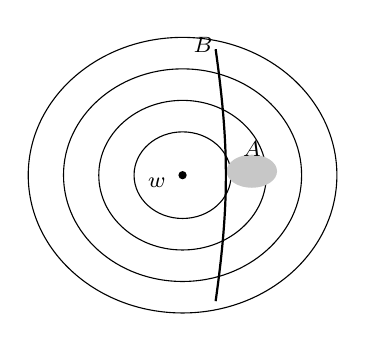
\begin{tikzpicture}[scale=1.0]
  \foreach \r in {0.55,0.95,1.35,1.75}{
    \draw[thin] (0,0) ellipse ({1.12*\r} and {\r});
  }
  \fill (0,0) circle (1.5pt);
  \node[font=\footnotesize,anchor=east] at (-0.09,-0.10) {$w$};
  \fill[black!22] (0.88,0.05) ellipse (0.32 and 0.21);
  \node[font=\footnotesize] at (0.88,0.33) {$A$};
  \draw[thick] (0.42,-1.6) to[out=82,in=278] (0.42,1.6);
  \node[font=\footnotesize] at (0.26,1.66) {$B$};
\end{tikzpicture}
\renewcommand{\thefigure}{7.7}
\caption{Lewis 最近世界语义的图形表示。每个椭圆区域对应一组与 $w$ 同等相似的世界。阴影区域表示最近 $A$ 世界的集合；由于这些世界全都满足 $B$，反事实语句 $A\cfs B$ 在 $w$ 中被判为真。}
\end{figure}

这一语义仍未解决表示问题。何种相似性度量的选择能使反事实推理与日常的因果观念相容？何种关于世界排序的心智表示能使反事实的计算（无论对人还是对机器）变得可操作、可实践？

在最初的提议中，Lewis 谨慎地让形式系统尽可能一般：除了要求每个世界离自己最近，他没有对相似性度量施加任何结构。然而简单的观察告诉我们，相似性度量不可能是任意的。人们能用反事实交流，这一事实本身已表明他们共享某种相似性度量，表明该度量被经济地编码于心智之中，因而必定高度结构化。Kit Fine (1975) 进一步表明，外观上的相似性并不充分。Fine 考虑反事实“若 Nixon 按下按钮，就会爆发核战争”——它一般被接受为真。显然，一个按钮恰好断线的世界，按我们所知，比一个产生核爆炸的世界与我们的世界相似得多。于是我们看到：相似性度量不仅不能任意，还必须尊重我们关于因果律的观念。\footnote{就此而言，Lewis 把原因约化为反事实的做法有点循环。} Lewis (1979) 随后在相似性的各个方面——“奇迹”（对定律的违反）的大小、事实的匹配、时间在先性等等——之间建立起一套错综的权重与优先序，试图让相似性更贴近因果直觉。但这些优先序相当事后，仍会得出反直觉的推断（J. Woodward，私人通信）。

这些困难在结构式说明中不会出现。与 Lewis 的理论相反，反事实并不基于假设世界之间相似性的抽象概念，而是直接建立在产生这些世界的机制（说得花哨些，即“定律”）以及这些机制的不变性质之上。Lewis 难以捉摸的“奇迹”，被有原则的微型手术 $\doop(X=x)$ 取代；后者表示确立前件 $X=x$（对一切 $u$）所必需的（对模型的）最小改动。

因此，相似性与优先序——若终究需要——可以作为事后的补充读入 $\doxp(\cdot)$ 算子（见 \textup{(3.11)} 之后的讨论以及 Goldszmidt and Pearl 1992），但它们不是分析的基础。

结构式说明以下述方式回答心智表示问题：它给出一种经济的知识编码，从中可以通过有效算法导出原因、反事实以及反事实的概率。然而，这种有效性部分是以把反事实前件限于基本命题的合取为代价换来的。析取式假设，例如“若 Bizet 与 Verdi 是同乡”，通常导致多重解，从而给出不唯一的概率赋值。

\subsection{公理比较}

若我们对世界间距离的评估来自因果知识，那么问题便是：这种知识是否会把自身的结构强加于距离之上——一种 Lewis 逻辑未曾刻画的结构？换个说法：若我们同意按因果关系度量世界的接近程度，是否会限制我们视为有效的反事实语句集合？这个问题不只是理论上的。例如，Gibbard and Harper (1976) 用 Lewis 的一般框架刻画决策条件句（即“若我们做 $A$，则 $B$”形式的语句），而我们的 $\doxp(\cdot)$ 算子建立在表示因果机制的函数之上；两个形式系统是否同一，尚不确定。\footnote{Ginsberg and Smith (1987) 与 Winslett (1988) 也提出了基于最近世界语义的行动理论；他们没有对距离度量施加任何特殊结构以反映因果考量。Pearl (2010c) 讨论了 $\doop(A\ \text{或}\ B)$ 的反事实解释。}

现在我们要证明：对递归系统而言，两个形式系统是同一的；换言之，只要递归性成立，复合性与实效性在 Lewis 的最近世界框架下也成立。我们先给出 Lewis 反事实语句逻辑的一个版本（取自 Lewis 1973c）。

\medskip
\noindent\textbf{规则}
\begin{enumerate}[label=(\arabic*),leftmargin=2.4em]
\item 若 $A$ 与 $A\cfs B$ 是定理，则 $B$ 是定理。
\item 若 $(B_1\ \&\ \cdots)\Rightarrow C$ 是定理，则 $\bigl((A\cfs B_1)\cdots\bigr)\Rightarrow(A\cfs C)$ 是定理。
\end{enumerate}

\medskip
\noindent\textbf{公理}
\begin{enumerate}[label=(\arabic*),leftmargin=2.4em]
\item 一切真值函项重言式。
\item $A\cfs A$。
\item $(A\cfs B)\ \&\ (B\cfs A)\ \Longrightarrow\ \bigl((A\cfs C)\equiv(B\cfs C)\bigr)$。
\item $\bigl((A\vee B)\cfs A\bigr)\ \vee\ \bigl((A\vee B)\cfs B\bigr)\ \vee\ \Bigl(\bigl((A\vee B)\cfs C\bigr)\equiv\bigl((A\cfs C)\ \&\ (B\cfs C)\bigr)\Bigr)$。
\item $(A\cfs B)\ \Longrightarrow\ (A\Rightarrow B)$。
\item $(A\ \&\ B)\ \Longrightarrow\ (A\cfs B)$。
\end{enumerate}

语句 $A\cfs B$ 表示“在 $A$ 成立的一切最近世界中，$B$ 也成立”。为把 Lewis 的公理与因果模型的公理联系起来，我们必须翻译他的句法。我们将把 Lewis 的“世界”等同于因果模型中一切变量（包括 $U$ 中的变量）的一个实例化。因果模型中对变量子集所作的赋值，将代表 Lewis 的命题（即上述规则与公理中的 $A$ 与 $B$）。于是，令 $A$ 表示合取 $X_1=x_1,\dots,X_n=x_n$，$B$ 表示合取 $Y_1=y_1,\dots,Y_m=y_m$。则
\begin{equation}
\begin{aligned}
A\cfs B\ \equiv\ & \bigl(Y_{1x_1,\dots,x_n}(u)=y_1\bigr)\\
&\&\ \bigl(Y_{2x_1,\dots,x_n}(u)=y_2\bigr)\\
&\&\ \cdots\\
&\&\ \bigl(Y_{mx_1,\dots,x_n}(u)=y_m\bigr).
\end{aligned}\tag{7.41}
\end{equation}
反之，我们需要把 $Y_x(u)=y$ 这样的因果语句翻译为 Lewis 的记号。令 $A$ 表示命题 $X=x$，$B$ 表示命题 $Y=y$。则
\begin{equation}
Y_x(u)=y\ \equiv\ A\cfs B. \tag{7.42}
\end{equation}

公理 (1)—(6) 由最近世界解释推出，除要求每个世界 $w$ 离自己不比任何其他世界 $w'\ne w$ 更远之外，并未对距离度量施加任何限制。由于结构语义在世界之间定义了一个显明的距离度量 $d(w,w')$——即把 $w$ 变换为 $w'$ 所需的局部干预的最少次数——Lewis 的一切公理都应在因果模型中成立，并且必须逻辑地由实效性、复合性以及（对非递归系统）可逆性推出。这一点将先予明确展示。然而，为保证结构语义不引入新的约束，我们还须证明其逆：结构语义的三条公理可由 Lewis 的公理推出。这一点随后展示。

为表明公理 (1)—(6) 在结构语义中成立，我们逐条考察。

(1) 该公理平凡为真。

(2) 该公理即实效性：若我们强制变量集 $X$ 取值 $x$，则 $X$ 的结果值为 $x$。即 $X_x(u)=x$。

(3) 该公理是可逆性的较弱形式，只对非递归因果模型有意义。

(4) 由于结构模型中的行动被限于文字（literal）的合取，该公理不相关。

(5) 该公理由复合性推出。

(6) 该公理由复合性推出。

为表明复合性与实效性可由 Lewis 的公理推出，我们注意到：在 Lewis 的形式系统中，复合性是公理 (5) 与规则 (1) 的推论，而实效性即 Lewis 的公理 (2)。

总之，对递归模型而言，因果模型框架并未在 Lewis 框架所施加的限制之外，对反事实语句增添任何限制；最近世界这一极为一般的概念已经足够。换个说法：递归性假设强到已经蕴含结构语义所施加的一切其他限制。然而考察非递归系统时我们会看到，可逆性并不由 Lewis 框架强制。Lewis 的公理 (3) 与可逆性相似但并不一样强：即使 $Y=y$ 在一切最近的 $w$ 世界中成立、$W=w$ 在一切最近的 $y$ 世界中成立，$Y=y$ 仍可能不在现实世界中成立。尽管如此，我们可以放心地结论：采用反事实的因果解释（连同可修改结构方程模型的表示与算法机械），并未对相对于递归系统有效的反事实语句集合引入任何限制。

\subsection{映像与条件化}

若行动是从一个概率函数到另一个概率函数的变换，人们可以问：是否每个这样的变换都对应某个行动？或者，源于行动的变换是否受某些特有约束？Lewis (1976) 对反事实的表述确实识别出这样的约束：变换必须是\emph{映像}（imaging）算子。

Bayes 条件化 $P(s\mid e)$ 把被 $e$ 排除的状态的全部概率质量转移到其余状态（按它们当前的 $P(s)$ 成比例）；映像则不同：每个被排除的状态 $s$ 各自把质量转移到一个精选的状态集 $S^*(s)$，这些状态被视为“最接近”$s$。确实，我们在 \textup{(3.11)} 中看到，由行动 $\doop(X_i=x_i')$ 定义的变换可以用这种质量转移过程来解释：每个被排除的状态（即 $X_i\ne x_i'$ 的状态）把质量转移到一个精选的未排除状态集，这些状态共享相同的 $\pa_i$ 取值。对最近状态集 $S^*(s)$ 的这种简单刻画对马尔可夫模型有效，但映像一般允许选取任何这样的集合。

映像为何更适合表示与行动相联系的变换，可从 Gardenfors (1988, thm.~5.2, p.~113；奇怪的是，Gardenfors 的分析中从未出现与行动的联系) 的一个表示定理看出。Gardenfors 的定理说：概率更新算子 $P(s)\mapsto P_A(s)$ 是映像算子，当且仅当它保持混合，即
\begin{equation}
\bigl[\alpha P(s)+(1-\alpha)P'(s)\bigr]_A=\alpha P_A(s)+(1-\alpha)P'_A(s) \tag{7.43}
\end{equation}
对一切常数 $1>\alpha>0$、一切命题 $A$、以及一切概率函数 $P$ 与 $P'$ 成立。换言之，任何混合的更新等于更新的混合。\footnote{性质 \textup{(7.43)} 反映在 Katsuno and Mendelzon (1991) 的 (U8) 公设中：$(K_1\circ K_2)o\mu=(K_1 o\mu)\vee(K_2 o\mu)$，其中 $o$ 是更新算子，类似于我们的 $\doxp(\cdot)$ 算子。}

这一性质称为同态性（homomorphy），它使我们能用转移概率来指定行动——这正是随机控制与马尔可夫决策过程中的惯常做法。记 $P_A(s\mid s')$ 为在已知状态 $s'$ 上施行 $A$ 所得的概率，则同态性 \textup{(7.43)} 要求
\begin{equation}
P_A(s)=\sum_{s'}P_A(s\mid s')\,P(s'); \tag{7.44}
\end{equation}
这意味着：当 $s'$ 不被确定地知道时，$P_A(s)$ 由 $P_A(s\mid s')$ 对 $s'$ 的加权和给出，权重为当前概率函数 $P(s')$。

然而这一刻画过于宽松：它虽然要求任何基于行动的变换都可用转移概率描述，却也把任何异想天开的转移概率设定都接受为某个行动的描述。行动被定义为局部手术这一宝贵信息，在此刻画中被忽略了。例如，与原子行动 $A_i=\doop(X_i=x_i)$ 相联系的转移概率，源自整个装配中仅仅一个机制的删除。因此，与各原子行动相联系的转移概率通常会相互约束。当概率被赋予 $U$ 的各个状态时，这类约束便从实效性、复合性与可逆性公理中浮现（Galles and Pearl 1997）。

\subsection{与 Neyman–Rubin 框架的关系}

\subsubsection*{一个寻找模型的语汇}

我们用来表示反事实量的记号 $Y_x(u)$，借自 Neyman (1923) 与 Rubin (1974) 的潜在结局框架——\S 3.6.3 已简要介绍，该框架是为处理效应的统计分析而设计的。\footnote{经济学中曾使用一个相关（若非同一）的框架：切换回归。关于此类模型的简要评述见 Heckman (1996；另见 Heckman and Honoré 1990 与 Manski 1995)。Winship and Morgan (1999) 对这两个学派作了出色的综述。}在该框架中，$Y_x(u)$（常写作 $Y(x,u)$）表示实验单元 $u$（如个人或一块农田）在假设性实验条件 $X=x$ 下的结局。然而与结构建模不同，这一变量并非从因果模型或任何科学知识的形式表示中导出，而是被当作原初概念——即一个未观测变量，只有当 $x$ 与实际接受的处理一致时才显露其值，如一致性规则（式 \textup{(7.20)}）所规定。因此，潜在结局框架不提供一个数学模型，使这类规则可从中导出，或使人们能据以尝试公理化刻画，以判定（例如）是否应引入附加规则，或某组潜在结局表达式是否冗余或矛盾。

\S 7.1 所表述的结构方程模型，恰恰提供了潜在结局框架所缺的形式语义：每个这样的模型都为潜在结局研究中所用的反事实量赋予连贯的真值。从结构视角看，$Y_x(u)$ 不是原初概念，而是从方程组 $F$ 数学地导出；$F$ 透明地表示了我们关于所论主题的知识。这种知识通过参与方程的变量定性地表达，无须承诺其精确的函数形式。变量 $U$ 表示与分析相关的任一背景因素集，未必是总体中某个具体个人的身份。

利用这一语义，我们在 \S 7.3 中建立了潜在响应函数 $Y_x(u)$ 及其与被观测变量 $X(u)$、$Y(u)$ 之关系的公理化刻画。这些基本公理包含或蕴含诸如一致性规则（式 \textup{(7.20)}）这样的限制，而潜在结局研究者把这些限制当作给定。

完备性结果进一步保证：递归模型中涉及反事实关系的推导，只需实效性与复合性两条公理便可安全处理。结构方程语义所蕴含的一切真理，也都可用这两条公理导出。同样地——在构造递归模型的假设性列联表时（见 \S 6.5.3）——我们得到保证：一旦某张表满足实效性与复合性，就至少存在一个因果模型能生成该表。这在本质上确立了结构方程建模（在经济学与社会科学中流行，Goldberger 1991）与统计学中所用的潜在结局框架（Rubin 1974; Holland 1986; Robins 1986）的形式等价性。\footnote{这一等价性在 Holland (1988)、Pratt and Schlaifer (1988)、Pearl (1995a) 与 Robins (1995) 中已被预见，并通过式 \textup{(3.51)} 的显式翻译及随后的定理 7.3.6 完备性结果而成为数学事实。}然而在非递归模型中，情况并非如此：仅用复合性与实效性来评估反事实语句，可能会漏证某些有效结论（即在一切因果模型中为真），而这些结论的有效性只有借助可逆性才能被识别。

\subsubsection*{图形分析与反事实分析}

结构框架与潜在结局框架之间的这一形式等价性，涉及语义与表达力的问题，却不意味着概念化或实用价值上的等价。结构方程及其相联的图，作为表达因果假设的手段特别有用。这类假设依托于先前的经验知识；大量证据表明，这种知识以相互联系的自主机制之装配的形式编码于人心。因此，这些机制是推导反事实判断的构件。结构方程 $\{f_i\}$ 及其图形抽象 $G(M)$ 为这些机制提供了直接的映射，因而构成一种自然语言，用以表述或验证因果知识或假设。潜在结局框架的主要弱点在于：它要求把假设表述为涉及反事实变量的条件独立关系。例如，\textup{(7.30)} 所表达的假设即使对熟练的研究者也难以理解，而它的结构映像 $U_1\indep U_2$ 却立刻唤起基于过程的解释。\footnote{这些看法与 Angrist 等 (1996) 所表达的观点截然相反，他们写道：“通常研究者对于这些扰动项究竟代表什么并没有明确的想法。”各领域的行家对这些扰动项代表什么有非常清楚的想法；而没有这种认识的人，肯定无法对反事实依赖性作出切合实际的判断。确实，回避结构方程或图的研究者，其分析往往也回避主题知识（如 Rubin 2009）。}

图形与反事实记号之间的良性共生，已在 \S 7.3.2 中演示。在该例中，假设先以图形形式表达，再（用 \textup{(7.25)} 与 \textup{(7.26)} 的规则）翻译为反事实记号，最后交由代数推导。这种共生比坚持把假设直接表述为反事实的方法更为有效。更多例子将在第九章分析因果概率时演示。注意，在 \S 7.3.2 的推导中，图还通过显示那些单靠代数手段不易导出的独立关系，持续辅助整个过程。例如，要证明 \textup{(7.27)}—\textup{(7.30)} 的假设蕴含条件独立 $(Y_z\indep Z_x\mid\{Z,X\})$ 却不蕴含条件独立 $(Y_z\indep Z_x\mid Z)$，并不简单。然而这类蕴含关系可以很容易地在图 7.5 或 \S 7.1.3 的孪生网络构造（见图 7.3）中检验。

用图的语言塑造因果假设，最有力的理由是：这类假设需要在数据收集之前、在模型参数仍然“自由”（即仍待由数据确定）的阶段给出。通常的诱惑是用统计独立的语言来塑造这些假设，因为它带有可检验性、从而带有科学合法性的光环。（第六章例示了这种诱惑的无益。）然而，统计独立的条件——无论涉及 $V$ 变量、$U$ 变量还是反事实——一般都敏感于模型参数的取值，而这些参数在建模阶段尚不可得。建模阶段可得的实质知识无法支持这类假设，除非它们是\emph{稳定的}，即对所涉参数的取值不敏感。图形模型的蕴含关系仅依托机制之间的相互联系，满足这一稳定性要求，因而可以在数据收集之前从一般的实质知识中确定。例如，图 7.5 的图所蕴含的断言 $(X\indep Y\mid Z,U_1)$，对 $\{f_i\}$ 中函数的任何替换、以及对 $U_1$ 与 $U_2$ 的任何先验概率赋值，都依然成立。

这些考量不仅适用于因果假设的表述，也适用于定义与交流因果概念所用的语言。社会科学与医学中的许多概念，是用未观测的 $U$ 变量（又称“误差”或“扰动项”）之间的关系来定义的。我们在第五章（\S 5.4.3）已看到，外生性与工具变量等关键计量经济学概念，传统上是用某些被观测变量与某些误差项之间不存在相关来定义的。自然，这类定义招致严格经验主义者的批评，他们把不可观测量视为形而上学或定义性的东西（Richard 1980; Engle et al. 1983; Holland 1988）；近来也招致潜在结局分析者的批评，他们错误地把使用结构模型视为对特定函数形式的不当承诺（Angrist et al. 1996）。这一批评将在下一节讨论。

\subsection{外生性与工具：反事实定义与图形定义}

本章的分析为结构方程模型中的误差项提供了反事实解释，补充了 \textup{(5.25)} 的操作定义。我们已看到，方程 $Y=f_Y(\pa_Y,u_Y)$ 中误差项 $u_Y$ 的含义，由反事实变量 $Y_{\pa_Y}$ 捕捉。换言之，变量 $U_Y$ 可解释为从 $\PA_Y$ 到 $Y$ 的函数映射的修饰因子。这类修饰的统计性质在 $\pa_Y$ 固定时可观测。这一翻译为反事实记号，可能有助于对 $U_Y$ 作代数处理而无须承诺 $f_Y$ 的函数形式。不过，从模型设定的角度看，误差项仍应被视为（被省略因素的）汇总。

有了这一解释，我们便能为原先以误差为基础定义的因果概念，取得图形定义与反事实定义。这类概念的例子有因果影响、外生性与工具变量（\S 5.4.3）。在澄清这些概念的误差基础定义、反事实定义与图形定义之间的关系时，我们首先应注意：这三种描述方式可以组织成一个简单的层级。由于图分离蕴含独立，而独立不蕴含图分离（定理 1.2.4），基于图分离的定义应蕴含基于误差项独立的定义。同样，由于对任意两个变量 $X$ 与 $Y$，独立关系 $U_X\indep U_Y$ 蕴含反事实独立 $X_{\pa_X}\indep Y_{\pa_Y}$（反之不然），基于误差独立的定义应蕴含基于反事实独立的定义。总体而言，我们有如下层级：
\[
\text{图形判据}\ \Longrightarrow\ \text{误差判据}\ \Longrightarrow\ \text{反事实判据}.
\]

外生性概念可用来说明这一层级。外生性的实用定义最好用反事实或干预的术语表述如下。

\medskip
\noindent\textbf{外生性（反事实判据）}\quad 变量 $X$ 相对于 $Y$ 是外生的，当且仅当 $X$ 对 $Y$ 的效应等同于给定 $X$ 时 $Y$ 的条件概率——即若
\begin{equation}
P(Y_x=y)=P(y\mid x), \tag{7.45}
\end{equation}
或等价地，
\begin{equation}
P(Y=y\mid\doop(x))=P(y\mid x); \tag{7.46}
\end{equation}
这又等价于独立条件 $Y_x\indep X$，Rosenbaum and Rubin (1983) 称之为“弱可忽略性”。\footnote{本节把讨论集中于外生性的因果成分，计量经济学文献不幸把它改名为“超外生性”（见 \S 5.4.3）。流行病学家把 \textup{(7.46)} 称为“无混杂”（见 \textup{(6.10)}）。我们还将“强可忽略性”——定义为联合独立 $\{Y_x,Y_{x'}\}\indep X$——的讨论推迟到第九章（定义 9.2.3）。}

这一实用的定义之所以实用，是因为它凸显了经济学家何以应当关心外生性：它阐明了发现某变量为外生所具有的政策分析收益。然而，这一定义未能引导研究者从领域的实质知识出发，去验证该独立条件在任何给定系统中是否成立，尤其当涉及许多方程时（见 \S 11.3.2）。为便于此类判断，经济学家（如 Koopmans 1950; Orcutt 1952）采用了定义 5.4.6 的误差判据。

\medskip
\noindent\textbf{外生性（误差判据）}\quad 若 $X$ 独立于一切对 $Y$ 有（不经 $X$ 中介的）影响的误差项，则称 $X$ 在 $M$ 中相对于 $Y$ 是外生的。\footnote{文献中有时要求相对于一切误差独立（如 Dhrymes 1970, p.~169），但这显然太强。}

这一定义对人类判断更透明，因为提及误差项会把注意力引向科学家所熟悉的、可能影响 $Y$ 的具体因素。不过，要判断这些因素是否统计独立，仍是一项艰难的心智任务，除非所考虑的独立关系由拓扑考量所支配，从而保证其稳定性。确实，最流行的外生性观念概括在“共同原因”这一概念中；它可以形式地表述如下。

\medskip
\noindent\textbf{外生性（图形判据）}\quad 若 $X$ 与 $Y$ 在 $G(M)$ 中没有共同祖先，或等价地，若 $X$ 与 $Y$ 之间的一切后门路径都被（对撞箭头）阻断，则 $X$ 相对于 $Y$ 是外生的。\footnote{如第六章（注 19）那样，“共同祖先”一语应排除那些除经由 $X$ 外与 $Y$ 没有其他联系的节点，并应为每一对相依误差引入潜节点。相对于被观测协变量的条件外生性的推广，在三种定义中都很直接。}

容易证明：图形条件蕴含误差判据，后者又蕴含 \textup{(7.46)} 的反事实（或实用）判据。反之不成立。例如，图 6.4 例示了图形判据失效、而误差判据与反事实判据都把 $X$ 归为外生的情形。我们在 \S 6.4 中论证，这类外生性（那里称为“无混杂”）是不稳定的或偶然的，并提出了这类情形是否本应被定义所涵盖的问题。若把不稳定情形排除在外，我们的三层级便坍缩，三种定义重合。

\subsubsection*{工具变量：三种定义}

工具变量概念同样具有三层级结构（Bowden and Turkington 1984; Pearl 1995c; Angrist et al. 1996），示于图 5.9。传统定义把变量 $Z$ 称为（相对于对 $(X,Y)$ 的）工具，若 (i) $Z$ 独立于一切对 $Y$ 有（不经 $X$ 中介的）影响的变量（包括误差项），且 (ii) $Z$ 与 $X$ 不独立。

反事实定义\footnote{事实上，工具变量向非线性系统的推广尚无共识。这里的定义取自 Galles and Pearl (1998)，其做法是把误差判据翻译为反事实语汇。Angrist 等 (1996) 明确拒斥一切对图或误差项的提及，却假定了两条不必要的限制：$Z$ 可忽略（即随机化；这在图 7.8(b) 与 (c) 中被违反），以及 $Z$ 影响 $X$（这在图 7.8(c) 中被违反）。Heckman and Vytlacil (1999) 作了类似假定，他们同时使用反事实与结构方程模型。回避图是有风险的。}把条件 (i) 替换为 (i$'$)：$Z$ 与 $Y_x$ 独立。图形定义把条件 (i) 替换为 (i$''$)：连接 $Z$ 与 $Y$ 的每条未阻断路径都必须含一个指向 $X$ 的箭头（等价地，$(Z\indep Y)_{G_{\underline{X}}}$）。图 7.8 用例子说明了这一定义。

\begin{figure}[htbp]
\centering
\begin{tikzpicture}[causal,scale=0.88,every node/.style={transform shape},
  vtxs/.append style={font=\scriptsize,minimum size=6.4mm,inner sep=0.5pt},
  lat/.append style={font=\scriptsize,minimum size=7.2mm,inner sep=0.5pt}]
  % ---- (a) ----
  \begin{scope}[xshift=0cm]
    \node[vtxs] (a1) at (0,1.35) {$Z$};
    \node[vtxs] (a2) at (0,0.15) {$X$};
    \node[vtxs] (a3) at (0,-1.05) {$Y$};
    \node[lat,minimum size=4.4mm] (a4) at (1.15,0.15) {};
    \node[font=\scriptsize,anchor=west] at (1.32,0.26) {$U_Y$};
    \draw[ed]  (a1) -- (a2);
    \draw[ed]  (a2) -- (a3);
    \draw[edd] (a4) -- (a3);
    \draw[bid] (a2) to[out=48,in=132] (a4);
    \node[font=\footnotesize] at (0.55,-1.6) {(a)};
  \end{scope}
  % ---- (b) ----
  \begin{scope}[xshift=3.7cm]
    \node[vtxs] (b1) at (0,1.35) {$Z$};
    \node[vtxs] (b2) at (0,0.15) {$X$};
    \node[vtxs] (b3) at (0,-1.05) {$Y$};
    \node[lat,minimum size=4.4mm] (b4) at (1.15,0.15) {};
    \node[font=\scriptsize,anchor=west] at (1.32,0.26) {$U_Y$};
    \draw[ed]  (b1) -- (b2);
    \draw[ed]  (b2) -- (b3);
    \draw[edd] (b4) -- (b3);
    \draw[bid] (b2) to[out=48,in=132] (b4);
    \draw[bid] (b1) to[bend left=52] (b2);
    \node[font=\footnotesize] at (0.55,-1.6) {(b)};
  \end{scope}
  % ---- (c) ----
  \begin{scope}[xshift=7.4cm]
    \node[vtxs] (c1) at (0,1.35) {$Z$};
    \node[vtxs] (c2) at (0,0.15) {$X$};
    \node[vtxs] (c3) at (0,-1.05) {$Y$};
    \node[lat,minimum size=4.4mm] (c4) at (1.15,0.15) {};
    \node[font=\scriptsize,anchor=west] at (1.32,0.26) {$U_Y$};
    \node[lat,minimum size=4.4mm]   (c5) at (0.8,1.6) {};
    \draw[edd] (c5) -- (c1);
    \draw[edd] (c5) -- (c2);
    \draw[ed]  (c2) -- (c3);
    \draw[edd] (c4) -- (c3);
    \draw[bid] (c2) to[out=48,in=132] (c4);
    \node[font=\footnotesize] at (0.55,-1.6) {(c)};
  \end{scope}
  % ---- (d) ----
  \begin{scope}[xshift=11.1cm]
    \node[vtxs] (d1) at (0,1.4) {$Z$};
    \node[vtxs] (d2) at (0.9,0.55) {$X$};
    \node[vtxs] (d3) at (0.1,-0.7) {$W$};
    \node[vtxs] (d4) at (1.05,-1.55) {$Y$};
    \node[lat,minimum size=4.4mm] (d5) at (-1.05,0.2) {};
    \node[font=\scriptsize,anchor=south] at (-1.05,0.45) {$U_W$};
    \node[lat,minimum size=4.4mm] (d6) at (2.25,-0.45) {};
    \node[font=\scriptsize,anchor=west] at (2.42,-0.34) {$U_Y$};
    \draw[ed]  (d1) -- (d2);
    \draw[edd] (d5) -- (d3);
    \draw[ed]  (d1) to[out=-135,in=80] (d3);
    \draw[ed]  (d3) -- (d4);
    \draw[ed]  (d2) -- (d4);
    \draw[edd] (d6) -- (d4);
    \draw[bid] (d2) to[out=-25,in=135] (d6);
    \node[font=\footnotesize] at (0.55,-2.1) {(d)};
  \end{scope}
\end{tikzpicture}
\renewcommand{\thefigure}{7.8}
\caption{在 (a)、(b)、(c) 的模型中，$Z$ 是合格的工具变量，因为它满足 $Z\indep U_Y$；在 (d) 中它不是工具，因为它与 $W$ 相关，而 $W$ 影响 $Y$。}
\end{figure}

当测量到协变量集 $S$ 时，这些定义可推广如下。

\begin{definition}[工具]
若存在不受 $X$ 影响的测量集 $S=s$，使下列判据之一成立，则称变量 $Z$ 是相对于 $X$ 对 $Y$ 之总效应的\emph{工具}。
\begin{enumerate}[label=\arabic*.,leftmargin=1.9em]
\item \textbf{反事实判据}：
\begin{enumerate}[label=(\roman*),leftmargin=2.4em]
\item $Z\indep Y_x\mid S=s$；
\item $Z\nindep X\mid S=s$。
\end{enumerate}
\item \textbf{图形判据}：
\begin{enumerate}[label=(\roman*),leftmargin=2.4em]
\item $(Z\indep Y\mid S)_{G_{\underline{X}}}$；
\item $(Z\nindep X\mid S)_G$。
\end{enumerate}
\end{enumerate}
\end{definition}

在结束本节时，我应再次强调：正因为图形定义对模型参数的取值不敏感，图形语汇才能如此好地引导并表达我们关于因果效应、外生性、工具、混杂、乃至（我猜测）随机性与统计独立等更技术性概念的直觉。

\section{结构因果性与概率因果性}

概率因果性是哲学的一个分支，试图用概率关系阐明因果关系。这一尝试由若干想法与期待所驱动。首先也最重要的是，概率因果性承诺解决那个延续数百年的因果发现之谜——即人类如何从赤裸的经验观察中发现真正的因果关系，而不带任何因果成见。鉴于 Hume 的教条（一切知识都源于人类经验），以及（不那么有说服力但当时很时髦的）假定（人类经验以概率函数的形式编码），人们自然期待因果知识可约化为某个定义在所关心变量上的概率分布中的一组关系。第二，与因果性的确定性说明相比，概率因果性带来可观的认知经济性：物理状态与物理定律无须极细微地指定，因为可以把它们概括为宏观状态之间的概率关系，从而与自然话语的粒度相匹配。第三，概率因果性有能力处理现代（即量子理论的）不确定性观念：按此观念，决定论只是一种认识论的虚构，非确定性才是物理实在的根本特征。

概率因果性的形式纲领发端于 Reichenbach (1956) 与 Good (1961)，其后由 Suppes (1970)、Skyrms (1980)、Spohn (1980)、Otte (1981)、Salmon (1984)、Cartwright (1989) 与 Eells (1991) 推进。考虑到其初衷，该纲领的现状相当令人失望；但若想到我们在 \S 1.5 的讨论，也并不意外。Salmon 已完全放弃这一努力，其结论是“因果关系不适合用统计相关性关系来分析”（1984, p.~185）；他转而提出以“因果过程”为基本构件的分析。Cartwright 与 Eells 较近的说明解决了 Salmon 遇到的一些困难，但代价是要么把理论复杂到面目全非，要么牺牲其原初目标。以下是 Cartwright (1989) 与 Eells (1991) 所描绘的概率因果性之主要成就、困难与妥协的简要叙述。

\subsection{对时序的依赖}

因果性的标准概率说明假定：除概率函数 $P$ 之外，我们还得到分析中变量的时序。这可以理解，因为因果性是非对称关系，而统计相关性是对称的。缺少时间信息，就无法判定两个相依变量中哪一个是原因、哪一个是结果，因为凡由“$X$ 是 $Y$ 之原因”的模型所诱导的联合分布 $P(x,y)$，也可由“$Y$ 是 $X$ 之原因”的模型诱导。于是，任何推断“$X$ 是 $Y$ 之原因”的方法，按对称性也必推断“$Y$ 是 $X$ 之原因”。第二章已表明：确实，判定 DAG 中箭头方向至少需要三个变量；更严重的是，单凭概率信息无法定向任何箭头——除非加上稳定性或极小性这一（因果）假设。通过施加“结果绝不先于原因”的约束，对称性被打破，因果推断才得以开始。

依赖时间信息有其代价：它先验地排除了时序未良好定义的案例分析，或因过程在时间上重叠，或因它们（看似）瞬时发生。例如，人们必须放弃（用非受控方法）判定持续体育锻炼是否降低胆固醇水平，还是反过来低胆固醇水平增强了锻炼的欲望。同样，概率因果性的哲学理论不会试图区分“高旗杆导致长影子”与“长影子导致高旗杆”——就一切实际目的而言，所谓原因与结果同时发生。

我们已在第二章看到，若辅以极小性或稳定性假设，某些因果方向性判定可从无时间的统计信息中作出。然而这些假设暗中反映了物理过程的一般性质——不变性与自主性（见 \S 2.9.1）——它们正是结构因果进路的基础。

\subsection{循环性的危险}

尽管依赖时间在先，哲学家们为识别因果关系所设计的判据仍受明显的循环性之困：要判定事件 $C$ 是否为事件 $E$ 的原因，必须预先知道其他因素与 $C$、$E$ 的因果关系。这种循环性源于界定“背景语境”的需要——因果关系的评估在该语境下进行；因为“原因应提高其结果的概率”这一直觉观念，必须用“其他情况相同”这一条件加以限定。例如，“学习算术”提高通过科学考试的概率，但只有在我们保持学生年龄不变时才如此；否则，学习算术实际上可能降低通过考试的概率，因为它是年幼的标志。于是，给出下述定义似乎很自然。

\begin{definition}
若在某个背景语境 $K$ 中存在至少一个条件 $F$，使 $P(E\mid C,F)>P(E\mid\neg C,F)$，则事件 $C$ 与 $E$ 因果相关。\footnote{读者可把 $K$ 理解为变量集，$F$ 为对这些变量的某个真值赋值。}
\end{definition}

但背景语境中应包含何种条件？一方面，坚持对物理环境作完备描述，会把概率因果性化为确定性物理（除非考虑量子层面的因素）。另一方面，完全忽略背景因素——或把它们描述得过于粗糙——会引入伪相关与其他混杂效应。一个自然的折中是要求背景语境本身对所论变量“因果相关”，但这一举措正是概率因果性定义中循环性的来源。

选择合适的背景因素集，类似于寻找合适的混杂调整，正如前几章围绕 Simpson 悖论所讨论的（如 \S 3.3、\S 5.1.3 与 \S 6.1）。我们已看到（如 \S 6.1），选择合适协变量集作调整的判据不能仅基于概率关系，而必须依赖因果信息。特别地，我们必须确保列为背景的因素满足后门条件，因为定义 7.5.1 中的不等式总可以通过对某个想象的因素 $F$ 取条件而满足（如图 6.2(c)），该因素在 $C$ 与 $E$ 之间制造伪关联。这里便出现了循环性：为判定 $C$ 相对于 $E$ 的因果作用（如药物对康复的效应），我们必须先判定每个因素 $F$（如性别）相对于 $C$ 与 $E$ 的因果作用。

人们或可通过对 $C$ 之前的一切因素取条件来逃避这一循环，但不幸的是，另一些无法仅凭时序识别的因素也必须权衡。考虑 \S 7.2.2 所用的打赌例子。我必须在一次公平掷硬币的结果上押正面或反面；猜对即赢，猜错即输。自然，一旦硬币掷出（而结果仍未知），打赌便被视为与获胜因果相关，尽管无论押正面还是反面，获胜的概率都一样。为揭示打赌（$C$）的因果相关性，我们必须把硬币的结果（$F$）纳入背景语境，尽管 $F$ 并不满足共同原因判据——它既不影响我的打赌（$C$），也不与获胜（$E$）因果相关（除非我们先宣布打赌与获胜相关）。更糟的是，我们无法以 $F$ 早于 $C$ 发生为理由把它纳入背景，因为硬币在我打赌之前还是之后掷出，与当前问题全然无关。我们的结论是：单凭时间在先不足以识别合适的背景语境，即使求助于 Eells (1991) 所谓的“交互原因”——即（简化的）因素 $F$，它们 (i) 不受 $C$ 的因果影响，且 (ii) 与 $C$ 联合（或与 $\neg C$ 联合）提高 $E$ 的概率。

由于一切因果相关性定义都固有循环性，概率因果性不能被视为从时间—概率信息中提取因果关系的纲领；毋宁说，它应被视为验证一组所提议的因果关系是否与可得的时间—概率信息相容的纲领。更形式地说，设某人给我们一个概率分布 $P$ 与（完备）变量集 $V$ 上的时序 $O$。此外，$V$ 中每对变量集（如 $X$ 与 $Y$）都标注符号 $R$ 或 $I$，$R$ 表示“因果相关”，$I$ 表示“因果无关”。概率因果性所处理的，是检验所提议的 $R$ 与 $I$ 标注是否与对 $(P,O)$ 相容，以及是否与“原因既先于其结果、又提高其结果之概率”这一信条相容。

目前最先进的相容性检验基于 Eells (1991) 的相关性判据，它可转述如下。

\medskip
\noindent\textbf{相容性检验}\quad 对每个标注为 $R(X,Y)$ 的变量对，检验：
\begin{enumerate}[label=(\roman*),leftmargin=2.6em]
\item 在 $O$ 中 $X$ 先于 $Y$；且
\item 存在 $x$、$x'$、$y$，使对某个 $z\in Z$ 有 $P(y\mid x,z)>P(y\mid x',z)$，其中 $Z$ 是背景语境 $K$ 中的变量集，满足 $I(X,Z)$ 与 $R(Z,Y)$。
\end{enumerate}

这又引出若干新问题：
\begin{enumerate}[label=(\alph*),leftmargin=2.2em]
\item 对每个对 $(P,O)$，是否存在相容的标注？
\item 标注何时唯一？
\item 当相容标注存在时，是否有找出它的程序？
\end{enumerate}
尽管图形方法为这些问题提供了一些洞见（Pearl 1996），要点在于：由于循环性，概率因果性的使命已被改变——从发现变为相容性检验。

还应指出，用条件化来定义因果性的基本纲领，即使成功，也与“因果性是关于干预的神谕”这一自然观念相悖。该纲领先把因果关系 $P(E\mid\doop(C))$ 与认识论的条件化 $P(E\mid C)$ 混为一谈，再通过补救性的条件化步骤去除伪相关，得到 $P(E\mid C,F)$。相反，结构式说明直接用自然的不变量（即定义 7.1.2 中的子模型 $M_x$）来定义因果性；见定理 3.2.2 之后的讨论。

\subsection{以孩子为例挑战封闭世界假设}

概率因果性所依据的范式中最关键、也最站不住脚的一条，是假定人们拥有关于某领域一切相关变量的概率函数。这一假定使分析者无须担心未测量的伪原因——它们可能（在物理上）影响分析中的若干变量，却仍不为分析者所知。众所周知，这类“混杂因子”的存在可能逆转或抵消任何从概率中得出的因果结论。例如，观察者若不知道蚊子的作用，可能会断言“坏空气”是疟疾的原因；或断言气压计下降是下雨的原因；或断言赶路上班是上班迟到的原因，等等。由于这些混杂因子未被测量（甚至未被怀疑），上述例子中的混杂无法通过取条件或“把它们固定”来消除。因此，认真对待 Hume 从原始数据中提取因果信息的纲领，就意味着要应对这样一个问题：任何此类信息的有效性，都寄托在“一切相关因素均已被考虑”这一不可检验的假定之上。

这就提出一个问题：人们究竟如何从环境中获得因果信息？更具体地说，儿童如何从经验中提取因果信息？试图用统计学学习理论解释这一现象的概率因果性倡导者，不能忽视一个事实：儿童从来不在封闭、孤立的环境中活动。未被注意的外部条件支配着每个学习环境的运作，而这些条件常常可能以出人意料且隐秘的方式混淆因果。

幸运的是，儿童并非在封闭、无菌的环境中成长，这也有其好处。除被动观察外，儿童拥有两种普通统计学家所不具备的宝贵因果信息源：操纵性实验与语言指导。操纵使所谓因果事件只受一个已知机制的影响，从而压倒了其他可能产生所谓结果的不受控因素。“独立操纵的妙处当然在于：其他因素可以在不被识别的情况下保持恒定”（Cheng 1992）。这种独立性是这样达成的：让所关心的对象服从自己意志的任意摆布，以确保操纵不受任何可能产生所谓结果的环境因素影响。例如，儿童能推断摇晃玩具会产生响声，因为正是儿童的手——只受其意志支配——带来了玩具的摇晃以及随后的响声。自由操纵的任意性取代了随机化实验的统计概念，并把儿童动作产生的声音与不受控环境因素产生的声音区分开来。

但操纵性实验无法解释人类获得并拥有的全部因果知识，因为环境中的大多数变量并不服从直接操纵。第二种宝贵的因果知识来源是语言指导：关于事物运作方式的明确因果语句，我们从父母、朋友、教师与书本中获得，它们编码了历代人的操纵经验。这一因果信息源看似显然无趣，却可能解释了我们因果知识的大部分；而理解这种知识传递如何运作，绝非易事。为理解并吸收“玻璃碎了，因为你推了它”这样的因果语句，儿童必须已经拥有一个因果图式，使这类输入在其中说得通。若要进一步推断：推玻璃会让人生你的气而不是生你兄弟的气——尽管上一个杯子是他打碎的——则需要真正精密的推断机械。在多数儿童身上，这种机械大概是天生的（Gopnik et al. 2004）。

然而要注意，语言输入大体上是定性的；我们很少听到父母向孩子解释：把玻璃杯放在桌边会使破碎概率提高 2.85 倍。概率进路把这类定性输入嵌入一个人为的数值框架，而结构进路（\S 7.1）直接建立在我们从语言中获得并传递的定性知识之上。

\subsection{单一原因与一般原因}

在 \S 7.2.3 中我们看到，一般原因（如“饮毒芹导致死亡”）与单一原因（如“苏格拉底饮毒芹导致了他的死亡”）之间的区分，在理解解释的本性时起重要作用。我们也提到，单一因果（又称“殊型”或“单一事件”因果）概念在因果性的概率说明中尚未达到恰当的概念化或形式化。本节详述这些困难的性质，并得出结论：它们源于概率说明的基本缺陷。

在第一章（图 1.6）中我们表明，评估单一因果主张所需的知识取反事实或函数关系的形式，而这种知识无法从赤裸的统计数据中提取，即使数据来自受控实验。\S 7.2.2 把这一限制归因于维持反事实语句所需的信息之时间持久性（或不变性）——这种持久性在统计陈述中被（平均化）冲掉，即使统计陈述被时间信息与因果相关信息所充实。这一基本限制的表现形式在概率因果性文献中呈现出有趣的侧面，并引出了关于单一陈述与一般陈述之间关系的激烈争论（如见 Good 1961; Cartwright 1989; Eells 1991; Hausman 1998）。

按概率因果性的一条基本信条，原因应提高结果的概率。然而我们常常在条件概率 $P(y\mid x)$ 低于 $P(y\mid x')$ 时，仍判定事件 $x$ 是 $y$ 的原因。例如，疫苗（$x$）通常降低疾病（$y$）的概率，而我们常说（且医学上可验证）疫苗本身在某人 $u$ 身上导致了该疾病。这类反转对结构模型的学习者不成问题：他们可以把单一陈述解释为“若 $u$ 未曾接种疫苗（$x'$），则 $u$ 本会仍然健康（$y'$）”。这一反事实语句的概率可以很高，而条件概率 $P(y\mid x)$ 乃至 $P(y\mid\doop(x))$ 很低，所有概率都由同一结构模型求值（\S 9.2 给出这三个量之间的精确关系）。然而，这一反转对概率因果性的学习者却是创伤性的：他们出于各种理由不信任反事实——部分因为反事实带有决定论的气息（Kvart 1986, pp.~256—63），部分因为反事实被认为建立在摇摇欲坠的形式基础之上，“对此我们只有语义学的开端（借助可能世界上的测度装置）”（Cartwright 1983, p.~34）。

为调和概率提高与单一因果这两个概念，概率论者主张：只要足够仔细地考察任何判定 $x$ 为 $y$ 之原因的情景，我们总能找到一个子总体 $Z=z$，在其中 $x$ 提高 $y$ 的概率——即
\begin{equation}
P(y\mid x,z)>P(y\mid x',z). \tag{7.47}
\end{equation}
在疫苗例子中，我们或可把所愿的子总体认定为对疫苗有不良易感性的人；按定义，疫苗在该子总体中无疑会提高疾病的概率。奇怪的是，只有少数哲学家注意到：“不良易感”这类因素本身是反事实地定义的；而一旦允许对这类因素取条件，就等于打开了一扇隐秘的后门，把决定论与反事实信息偷偷带回分析之中。

反事实较为隐蔽的一次露面，或许出现在 Hesslow 关于避孕药的例子中（Hesslow 1976），\S 4.5.1 已讨论。设我们发现 Jones 夫人没有怀孕，并追问服用避孕药是否是她患血栓的原因。未怀孕妇女这一总体结果太粗糙，无法明确回答该问题。若 Jones 夫人属于“若非服药本会怀孕”的那一类妇女，则服药在她这个案例中可能反而降低了血栓概率，因为它防止了怀孕。反之，若她属于“无论是否服药都不会怀孕”的那一类，则服药无疑提高了血栓的机会。这个例子有启发性，因为这两类检验总体在英语中没有既定名称（不同于疫苗例中的“易感性”），必须用反事实语汇显式定义。一位妇女属于前一类还是后一类，取决于许多社会与情境上的偶然因素，这些因素通常未知，也不大可能构成某人的不变属性。尽管如此，我们认识到在评估避孕药是否为 Jones 夫人血栓之原因时，必须分别考虑这两类。

于是我们看到，处理殊型层面的因果性时无法回避反事实。概率论者坚持用无反事实的句法来定义殊型因果主张，结果所划出的子总体恰恰由反事实表达式界定：疫苗例中的“不良易感”，Jones 夫人案例中的“本不会怀孕”。\footnote{Cartwright (1989, chap.~3) 认识到可观察的划分（如怀孕）不足以支撑概率提高论题，但她没有强调：支撑该论题的更精细划分必然具有反事实性质。并非偶然的是，Cartwright 曾是主张把反事实排除出因果分析的坚决拥护者（Cartwright 1983, pp.~34—5）。}

当然，概率论者可以辩称：无须把子类 $Z=z$ 细化到确定性的极端，因为一旦找到满足 \textup{(7.47)} 的、能提高 $y$ 概率的子类，便可停止细化。这一论证近乎同义反复，除非它伴随形式化的程序：如何识别检验子总体 $Z=z$，如何从某个合理的人类知识模型（哪怕是假设性的）计算 \textup{(7.47)} 中的量。不幸的是，概率因果性文献对程序与表示问题保持沉默。\footnote{甚至 Eells (1991, chap.~6) 与 Shafer (1996)——他们努力在通往 $y$ 的世界实际轨迹中揭示概率提高的判别模式——也未指明：选择合适轨迹、或计算与给定轨迹相联的概率，需要什么信息。}

尤其地，概率论者在解释下述问题时面临艰难的两难：人们何以如此迅速而一致地寻找那个救场的子总体 $z$？当被问及“是否是 $x$ 导致了 $y$”时，多数人何以得出相同答案？例如（据 Debra Rosen，引自 Suppes 1970），一根偶然拨偏高尔夫球的树枝（$x$）会立即且一致地被看作球最终进洞的“原因”，尽管这类碰撞一般会降低进洞的机会（$y$）。显然，若此类例子中存在满足 \textup{(7.47)} 的子总体 $z$（我怀疑它是否曾进入任何人的头脑），它至少须有两个特征：
\begin{enumerate}[label=(\arabic*),leftmargin=2.2em]
\item 它必须包含既在 $x$ 之前、又在 $x$ 之后发生的事件。例如，球撞上树枝的角度，以及球撞枝后弹跳处草地的质地，都应属于 $z$。
\item 它必须依赖于 $x$ 与 $y$。因为，若我们要检验树枝是否导致了另一后果 $y'$——比如球在离洞两码处停下——\textup{(7.47)} 中显然需要不同的条件集 $z'$。
\end{enumerate}

这就把我们带到概率因果进路的一个重大方法论不一致：若对 $x$ 与 $y$ 的无知导致错误的 $z$，而对 $x$ 与 $y$ 的知晓导致正确地选择 $z$，那么必定存在某种过程，使人们把 $x$ 与 $y$ 的发生纳入其认知。这会是什么过程？按概率认识论的规范，证据通过条件化进入知识总体。那么，我们如何能正当地把导致 $z$ 之选择的证据本身——即 $x$ 与 $y$ 的发生——排除在 $z$ 之外？

考察 \textup{(7.47)} 可见，把 $x$ 与 $y$ 排除出 $z$ 是句法上的强制要求，否则会使 $P(y\mid x',z)$ 无定义，并使 $P(y\mid x,z)=1$。确实，在概率演算的句法中，我们不能问“已知 $y$ 事实上已经发生，事件 $y$ 的概率是多少”——答案是（平凡地）1。我们最多只能暂时脱离现实世界，假装不知道 $y$ 的发生，并在这种无知状态下追问 $y$ 的概率。这恰恰对应于支配 $P(Y_{x'}\ne y\mid x,y)$ 求值的三步（溯因、行动与预测）（见定理 7.1.7）；该量（在我们的例子中）取高值，并正确地把树枝（$x$）判定为使球进洞（$y$）的原因。如我们所见，所愿的量可以用对 $x$ 与 $y$ 的普通条件化来表达和求值，无须显式引入任何子总体 $z$。\footnote{所愿的子总体 $z$ 等于一切满足 $X(u)=x$、$Y(u)=y$ 且 $Y_x(u)=y'$ 的 $u$ 所构成的集合。}

具有讽刺意味的是，概率论者否认反事实条件句，结果却使自己无法使用标准条件句——正是他们试图保留的那些条件句——被迫以迂回方式容纳简单的证据信息。概率论者围绕因果性筑起的这道句法壁垒，在单一原因与一般原因之间造成了人为的紧张；而在结构式说明中，这种紧张消失了。在 \S 10.1.1 中我们将表明：一旦同时容纳标准条件句与反事实条件句（即 $Y_x$），单一原因与一般原因便不再需要分别分析。两类原因的区别仅在于带到问题之上的情景特定信息之多少，即进入量 $P(Y_x=y\mid e)$ 的证据 $e$ 的具体程度。

\subsection{小结}

Cartwright (1983, p.~34) 列出了若干理由，说明为何应采取概率进路而非反事实进路来研究因果性：

\begin{quote}
\kaishu
[反事实进路]要求我们求反事实的概率，而我们对此只有语义学的开端（借助可能世界上的测度装置），没有方法论，更谈不上说明该方法论为何与语义学相配。我们如何检验关于反事实概率的主张？我们没有答案，更谈不上有与初生语义学相符的答案。宁可要一种效力度量，它只要求实际世界中可按标准方式检验的事件概率。
\end{quote}

考察概率进路过去三十年的进展，似乎很清楚：Cartwright 的期望并未在她所主张的框架中实现，反而在与之竞争的反事实框架（体现于结构模型）中实现。用“可检验的事件”对“效力”（我们语汇中的“因果效应”）所作的完整刻画，源自 Simon (1953) 与 Strotz and Wold (1960) 关于可修改结构模型的概念，并在后门准则（定理 3.3.2）以及更一般的定理 3.6.1 与 4.4.1 中臻于成熟——概率判据（如 \textup{(3.13)}）不过是其粗糙的特例。用反事实概率 $P(Y_{x'}\ne y\mid x,y)$ 解释单一因果，已获得有意义的形式语义（\S 7.1）与有效的求值方法论（定理 7.1.7 与 \S 7.1.3—7.2.1）的支持；而 \textup{(7.47)} 的概率判据仍停留在模糊而无程序的争论中。一旦未观测量（如世界状态、背景语境、因果相关性、易感性）被允许渗入分析，概率框架便放弃了“使因果主张可检验”的原初梦想；而回答可检验性问题的方法论已转移到结构—反事实框架（见第九章与 \S 11.9）。

与非确定性物理学的教义保持相容，似乎是概率因果纲领仅存的可行方面；本节质疑：维护这一理想是否值得那些牺牲。本节还提示，概率因果纲领的基本议程该作一次严肃重估。若该纲领是认识论的一次演练，那么“概率的”一词便是矛盾修辞——人类对因果性的感知一直是准确定性的（quasi-deterministic），而这些易错的人类仍是因果话语的主要消费者。若该纲领是现代物理学的一次演练，那么“因果性”一词便非本质——量子层面的因果性遵循自己的规则与直觉，另取一名（也许叫“qua-sality”）或更贴切。不过，就人工智能与认知科学而言，我敢预言：被编程来模拟 Laplace 与 Einstein 的准确定性宏观近似的机器人，将远远胜过那些建立在 Born、Heisenberg 与 Bohr 正确却反直觉理论之上的机器人。

\section*{致谢}
\addcontentsline{toc}{section}{致谢}

本章若干节基于 Alex Balke 与 David Galles 的博士研究。这些研究受益于 Joseph Halpern 的投入甚多。
